\begin{activity} \label{A:1.7.1}
Consider a function that is piecewise-defined according to the formula
$$f(x) = \begin{cases}

  3(x+2)+2 & \text{for $-3 < x < -2$} \\
  \frac{2}{3}(x+2)+1 & \text{for $-2 \le x < -1$} \\
  \frac{2}{3}(x+2)+1 & \text{for $-1 < x < 1$} \\
  2 & \text{for $x = 1$} \\
  4-x & \text{for $x > 1$}

\end{cases}$$
Use the given formula to answer the following questions.
\begin{figure}[h]
\begin{center}
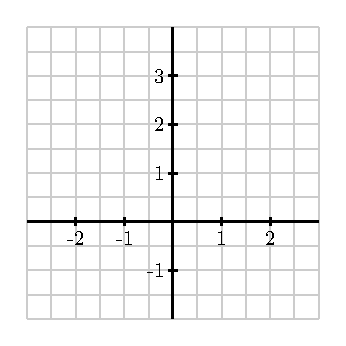
\includegraphics{figures/1_7_Act1.eps}
\caption{Axes for plotting the function $y = f(x)$ in Activity~\ref{A:1.7.1}.} \label{F:1.7.Act1}
\end{center}
\end{figure}
\ba
	\item For each of the values $a = -2, -1, 0, 1, 2$, compute $f(a)$.
	\item For each of the values $a = -2, -1, 0, 1, 2$, determine $\ds \lim_{x \to a^-} f(x)$ and $\ds \lim_{x \to a^+} f(x)$.  
	\item For each of the values $a = -2, -1, 0, 1, 2$, determine $\ds \lim_{x \to a} f(x)$.  If the limit fails to exist, explain why by discussing the left- and right-hand limits at the relevant $a$-value.
	\item For which values of $a$ is the following statement true?
	$$\lim_{x \to a} f(x) \ne f(a)$$
	\item On the axes provided in Figure~\ref{F:1.7.Act1}, sketch an accurate, labeled graph of $y = f(x)$.  Be sure to carefully use open circles ($\circ$) and filled circles ($\bullet$) to represent key points on the graph, as dictated by the piecewise formula.
\ea

\end{activity}
\begin{smallhint}
\ba
	\item Find the interval in which $a$ lies and evaluate the function there.
	\item Remember that for $\ds \lim_{x \to a^-} f(x)$, we only consider values of $x$ such that $x < a$.  Find the right formula to use in the piecewise definition for $f$ to fit the values you are considering.
	\item Use your work in (c) and compare left- and right-hand limits.
	\item Use your work in (a) and (c).
	\item Note that $f$ is piecewise linear.  
\ea
\end{smallhint}
\begin{bighint}
\ba
	\item Find the interval in which $a$ lies and evaluate the function there.  For example, $f(-2) = \frac{2}{3}(-2+2) + 1$, based on the formula for $f$.
	\item Remember that for $\ds \lim_{x \to a^-} f(x)$, we only consider values of $x$ such that $x < a$.  Find the right formula to use in the piecewise definition for $f$ to fit the values you are considering.  For example, as $x \to -2^-$, we use the formula $3(x+2)+2$ and see that $3(x+2)+2 \to 3(-2+2)+2 = 2$ as $x \to -2^+$.
	\item Use your work in (c) and compare left- and right-hand limits.  Remember that the overall limit exists if and only if both left and right limits exists and are equal in value.
	\item Use your work in (a) and (c).
	\item Note that $f$ is piecewise linear.  For instance, $y = 3(x+2) + 2$ is a line through $(-2,2)$ with slope 3 and is valid on the interval $-3 < x < -2$.
\ea\end{bighint}
\begin{activitySolution}
\ba
	\item $f(-2) = \frac{2}{3}(-2+2) + 1 = 1$; $f(-1)$ is not defined; $f(0) = \frac{2}{3}(0+2)+1 = \frac{7}{3}$; $f(1) = 2$ (by the rule); $f(2) = 4-2 = 2$.
	\item $$\lim_{x \to -2^-} f(x) = 2 \ \mbox{and} \lim_{x \to -2^+} f(x) = 1$$
	        $$\lim_{x \to -1^-} f(x) = \frac{5}{3} \ \mbox{and} \lim_{x \to -1^+} f(x) = \frac{5}{3}$$
	        $$\lim_{x \to 0^-} f(x) = \frac{7}{3} \ \mbox{and} \lim_{x \to 0^+} f(x) = \frac{7}{3}$$
	        $$\lim_{x \to 1^-} f(x) = 3 \ \mbox{and} \lim_{x \to 1^+} f(x) = 3$$
	        $$\lim_{x \to 2^-} f(x) = 2 \ \mbox{and} \lim_{x \to 2^+} f(x) = 2$$
	\item $\ds \lim_{x \to -2} f(x)$ does not exists because the left-hand limit is $2$ while the right-hand limit is $1$.  All of the other requested limits exist, as left- and right-hand limits exist and are equal in each case.  The respective values of the limits as $x \to a$ for $a = -1, 0, 1, 2$ are $\frac{5}{3}, \frac{7}{3}, 3, 2$.
	\item For $a = -2$, $a = -1$, and $a = 1$, $\ds \lim_{x \to a} f(x) \ne f(a)$.  At $a = -2$, the limit fails to exist, but $f(-2) = 1$.  At $a = -1$, the limit is $\frac{5}{3}$, but $f(-1)$ is not defined.  At $a = 1$, the limit is 3, but $f(1) = 2$.
	\item 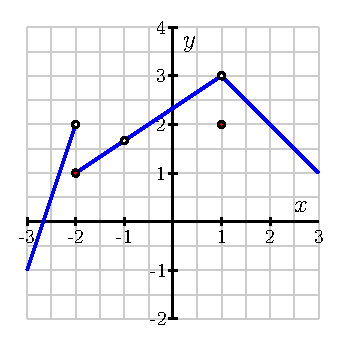
\includegraphics{figures/1_7_Act1Soln.eps}
\ea	        
\end{activitySolution}
\aftera